% Что пишем в программную реализацию?

% На каком языке программировании написано
\subsection*{Технология}
Описанная модель реализована на языке программирования Python. Реализация сочетает достоинства применения как парадигмы ООП, так и функционального программирования за счет активного использования лямбда-выражений.

% Какую библиотеку использовали
Для реализации на языке программирования был использован внешний модуль Pyomo [\ref{lit:22}]. В части решаемой задачи этот модуль был задействован для построения математической модели и взаимодействия с решателями [\ref{lit:22}, \ref{lit:23}]. Построение математической модели заключалось в динамической генерации параметров модели и ограничений. Взаимодействие с решателями - вызов их из переменных окружения среды, задание входных аргументов для их работы и считывание результатов вычислений.

% Раскрыть применение матрешки
\subsection*{Организация кода}
С целью понижения когнитивной сложности применяемого решения и достижения управляемости поведением каждой отдельной единицы функционала весь код разбит на обособленные модули, представленные в виде классов языка программирования Python.

Компоновка их друг с другом, последовательное разрешение зависимостей происходит в едином месте - в главной функции программы. В такой схеме отсутствуют передача локальных неуправляемых параметров по цепочке вызовов в иерархии функций, а каждая отдельная единица функционала работает в своем информационном окружении.

% Привести диаграмму вызовов или uml-диаграмму
Диаграмма классов приведена на рисунке \ref{fig:uml}.

% Рисунок uml-диагараммы
\begin{figure}[H]
    \centering
    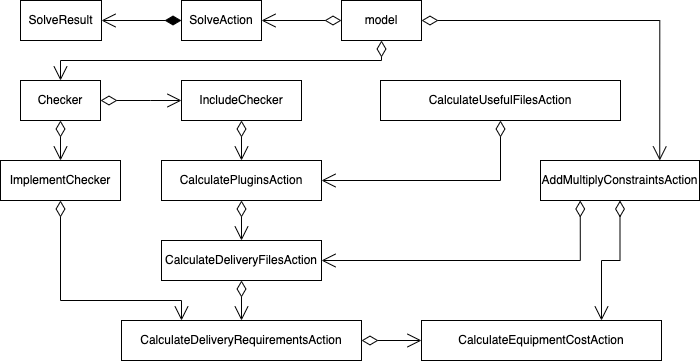
\includegraphics[width=1\textwidth]{uml}
    \caption{Диаграмма классов}
    \label{fig:uml}
\end{figure}
